\documentclass[12pt,a4paper]{article}

% ------------------------------------------------
% PAQUETES
% ------------------------------------------------

\usepackage[utf8]{inputenc}
\usepackage[T1]{fontenc}
\usepackage[spanish,es-nodecimaldot]{babel}

\usepackage{amsmath}
\usepackage{amssymb}

\usepackage{graphicx}
\usepackage{float}
\usepackage{booktabs}
\usepackage{array}
\usepackage{multirow}

\usepackage{hyperref}

\usepackage{geometry}
\geometry{
    top=2.5cm,
    bottom=2.5cm,
    left=2.8cm,
    right=2.8cm
}

\usepackage{setspace}
\onehalfspacing

\usepackage{parskip}

\usepackage{fancyhdr}
\pagestyle{fancy}
\fancyhf{}
\rhead{Cadena de Markov del caballo}
\lhead{Cadenas de Markov}
\cfoot{\thepage}

% ------------------------------------------------
% INFORMACIÓN DEL DOCUMENTO
% ------------------------------------------------

\title{
    \textbf{Cadena de Markov asociada al movimiento aleatorio de un caballo en un tablero de ajedrez \(8\times8\)}
}

\author{
    Henry Giovani Barrera Martínez
    Laura Victoria Torres Pinilla
}

\date{\today}

% ------------------------------------------------
% DOCUMENTO
% ------------------------------------------------

\begin{document}

% ------------------------------------------------
% PORTADA
% ------------------------------------------------

\begin{titlepage}

    \centering

    \vspace*{2cm}

    {\Large \textbf{Universidad Nacional de Colombia}\par}

    \vspace{0.5cm}

    {\large Departamento de Matemáticas\par}

    \vspace{2cm}

    {\LARGE
    \textbf{Cadena de Markov asociada al movimiento aleatorio de un caballo en un tablero de ajedrez \(8\times8\)}
    \par}

    \vspace{1.5cm}

    {\large Asignatura: Cadenas de Markov\par}

    \vspace{2cm}

    {\large
    \textbf{Estudiantes:}\\
        Henry Giovani Barrera Martínez\\
        Laura Victoria Torres Pinilla
    \par}

    \vfill

    {\large Bogotá D.C., Colombia\par}

    {\large \today\par}

\end{titlepage}

% ------------------------------------------------
% CONTENIDO
% ------------------------------------------------

\tableofcontents

\newpage

% ------------------------------------------------
% 1. INTRODUCCIÓN
% ------------------------------------------------

\section{Introducción}

Un caballo situado sobre un tablero de ajedrez \(8\times8\), que se
desplaza eligiendo uniformemente al azar uno de sus movimientos legales
en cada paso, define de manera natural una cadena de Markov con espacio
de estados finito: las 64 casillas del tablero. A diferencia de otras
aplicaciones clásicas de cadenas de Markov con dinámicas continuas o
espacios de estados muy grandes, este ejemplo tiene la ventaja de ser
completamente explícito y verificable: tanto el espacio de estados como
la matriz de transición pueden construirse y comprobarse por completo
mediante un programa.

Este informe desarrolla tres aspectos del problema. Primero, se
construye formalmente la cadena: el espacio de estados, los conjuntos
de vecindad \(N(x)\) y la matriz de transición \(P\), verificando
computacionalmente sus propiedades básicas. Segundo, se calculan
probabilidades concretas sobre trayectorias de la cadena, aplicando de
forma explícita la propiedad de Markov. Tercero, se estudia la
alcanzabilidad de estados mediante una exploración por niveles (BFS),
lo cual permite discutir formalmente la irreducibilidad y la
periodicidad de la cadena --- dos propiedades estructurales que
determinan su comportamiento a largo plazo.

% ------------------------------------------------
% 2. OBJETIVOS
% ------------------------------------------------

\section{Objetivos}

\subsection{Objetivo general}

Construir y analizar la cadena de Markov asociada al movimiento
aleatorio de un caballo en un tablero de ajedrez \(8\times8\),
determinando sus propiedades estructurales y calculando probabilidades
sobre trayectorias específicas.

\subsection{Objetivos específicos}

\begin{itemize}

    \item Definir el espacio de estados \(S\) y construir, para cada
    estado, el conjunto de vecindad \(N(x)\) y su cardinalidad
    \(|N(x)|\).

    \item Construir la matriz de transición \(P\) y verificar
    computacionalmente que define una matriz estocástica válida.

    \item Determinar si \(P\) es simétrica y justificar la respuesta
    distinguiendo la simetría de la relación de movimientos de la
    simetría de las probabilidades de transición.

    \item Calcular probabilidades de trayectorias específicas de la
    cadena a partir de \(X_0=a1\), aplicando la propiedad de Markov.

    \item Determinar, mediante una exploración por niveles, el conjunto
    de casillas alcanzables desde \(a1\) y desde \(d5\), y a partir de
    ello discutir la irreducibilidad de la cadena.

    \item Estudiar la periodicidad de la cadena a partir de la
    estructura bipartita del grafo de movimientos del caballo.

\end{itemize}

% ------------------------------------------------
% 3. CONSTRUCCIÓN DE LA CADENA
% ------------------------------------------------

\section{Construcción de la cadena de Markov}

\subsection{Espacio de estados}

Cada casilla del tablero se identifica mediante una letra de columna
\(a,\ldots,h\) y un número de fila \(1,\ldots,8\). El espacio de
estados es

\[
S=\{a1,a2,\ldots,a8,\;b1,\ldots,b8,\;\ldots,\;h1,\ldots,h8\},
\]

con

\[
|S|=64.
\]

Se fija el orden

\[
a1,a2,\ldots,a8,\,b1,\ldots,b8,\,\ldots,\,h1,\ldots,h8
\]

para indexar tanto los estados como las filas y columnas de la matriz
de transición.

\subsection{Movimientos del caballo y conjunto \(N(x)\)}

Desde una casilla \(x\), un caballo puede desplazarse mediante ocho
movimientos relativos posibles:

\[
(\pm1,\pm2),\qquad(\pm2,\pm1).
\]

El conjunto de vecindad se define como

\[
N(x)=\{y\in S: \text{existe un movimiento de caballo que lleva de }x\text{ a }y\},
\]

conservando únicamente los movimientos que permanecen dentro del
tablero. La Tabla~\ref{tab:vecindades-ejemplo} presenta una muestra
representativa de \(N(x)\) para distintos tipos de casilla (esquina,
borde y centro). La tabla completa para las 64 casillas se encuentra
en \texttt{results/tabla\_vecindades.csv}, generada automáticamente
por \texttt{src/tablero.py}.

\begin{table}[H]
\centering
\caption{Ejemplos representativos de \(N(x)\) y \(|N(x)|\).}
\label{tab:vecindades-ejemplo}

\begin{tabular}{clc}
\toprule
\(x\) & \(N(x)\) & \(|N(x)|\) \\
\midrule
\(a1\) (esquina) & \(\{b3,\,c2\}\) & 2 \\
\(h8\) (esquina) & \(\{g6,\,f7\}\) & 2 \\
\(b1\) (borde, junto a esquina) & \(\{c3,\,a3,\,d2\}\) & 3 \\
\(g1\) (borde) & \(\{h3,\,f3,\,e2\}\) & 3 \\
\(c1\) (borde) & \(\{d3,\,b3,\,e2,\,a2\}\) & 4 \\
\(h6\) (borde) & \(\{g8,\,g4,\,f7,\,f5\}\) & 4 \\
\(b3\) (interior, cercano al borde) & \(\{c5,\,c1,\,a5,\,a1,\,d4,\,d2\}\) & 6 \\
\(d4\) (centro) & \(\{e6,\,e2,\,c6,\,c2,\,f5,\,f3,\,b5,\,b3\}\) & 8 \\
\bottomrule
\end{tabular}

\end{table}

El valor \(|N(x)|\) depende únicamente de la posición de \(x\) respecto
a los bordes del tablero. Clasificando las 64 casillas según
\(|N(x)|\) se obtiene la distribución de la Tabla~\ref{tab:distribucion-N}.

\begin{table}[H]
\centering
\caption{Distribución del número de casillas según \(|N(x)|\).}
\label{tab:distribucion-N}

\begin{tabular}{cccccc}
\toprule
\(|N(x)|\) & 2 & 3 & 4 & 6 & 8 \\
\midrule
Número de casillas & 4 & 8 & 20 & 16 & 16 \\
\bottomrule
\end{tabular}

\end{table}

Las 4 casillas con \(|N(x)|=2\) corresponden exactamente a las cuatro
esquinas del tablero (\(a1,a8,h1,h8\)), mientras que las 16 casillas
con \(|N(x)|=8\) son las casillas centrales, suficientemente alejadas
de todos los bordes. La suma de las frecuencias es
\(4+8+20+16+16=64\), consistente con \(|S|=64\).

\subsection{Matriz de transición}

Dado que el caballo elige uniformemente entre sus movimientos legales,
la probabilidad de transición se define como

\[
P_{xy}=
\begin{cases}
\dfrac{1}{|N(x)|}, & y\in N(x),\\[4pt]
0, & y\notin N(x).
\end{cases}
\]

La matriz \(P\in\mathbb{R}^{64\times64}\) se construye
automáticamente a partir de \(N(x)\) (ver
\texttt{src/matriz\_transicion.py}). Se verificaron computacionalmente
las siguientes propiedades sobre las 64 filas:

\begin{itemize}
    \item \(P\) tiene dimensión \(64\times64\).
    \item Cada fila suma exactamente \(1\): \(\sum_{y\in S}P_{xy}=1\)
    para todo \(x\in S\).
    \item \(P_{xy}=0\) siempre que \(y\notin N(x)\), y
    \(P_{xy}=1/|N(x)|\) siempre que \(y\in N(x)\).
\end{itemize}

Las tres verificaciones se satisfacen para las 64 filas sin excepción,
confirmando que \(P\) es una matriz estocástica válida consistente con
su definición.

\subsubsection*{Filas solicitadas}

Las probabilidades de transición desde \(g1\) y \(h6\) son:

\[
P_{g1,y}=
\begin{cases}
\dfrac13, & y\in\{e2,\,f3,\,h3\},\\
0,& \text{en otro caso},
\end{cases}
\qquad
P_{h6,y}=
\begin{cases}
\dfrac14, & y\in\{f5,\,f7,\,g4,\,g8\},\\
0,& \text{en otro caso}.
\end{cases}
\]

\subsubsection*{Probabilidades pedidas en el numeral 1d}

\[
P_{h8,y}=\tfrac12 \text{ para } y\in\{f7,g6\},
\qquad
P_{g1,y}=\tfrac13 \text{ para } y\in\{e2,f3,h3\},
\]
\[
P_{b7,y}=\tfrac14 \text{ para } y\in\{a5,c5,d6,d8\},
\qquad
P_{f7,y}=\tfrac16 \text{ para } y\in\{d6,d8,e5,g5,h6,h8\},
\]
\[
P_{e5,y}=\tfrac18 \text{ para } y\in\{c4,c6,d3,d7,f3,f7,g4,g6\}.
\]

En cada caso, las casillas no listadas tienen probabilidad de
transición cero, y las probabilidades listadas suman \(1\), como exige
la definición.

\subsection{Simetría de \(P\)}

La matriz \(P\) \textbf{no} es simétrica. Es importante distinguir dos
nociones distintas:

\begin{itemize}
    \item La \emph{relación de movimientos} (¿puede el caballo pasar de
    \(x\) a \(y\)?) es simétrica: si el caballo puede moverse de \(x\)
    a \(y\), también puede moverse de \(y\) a \(x\), ya que los ocho
    desplazamientos relativos de caballo forman un conjunto cerrado
    bajo inversión de signo. En términos de grafos, el grafo de
    movimientos del caballo es \textbf{no dirigido}.

    \item Sin embargo, las \emph{probabilidades de transición} no
    heredan esta simetría, porque \(P_{xy}=1/|N(x)|\) depende del
    número de vecinos de \(x\), no del de \(y\).
\end{itemize}

Como contraejemplo explícito, para \(x=a1\), \(y=b3\):

\[
P_{a1,b3}=\frac{1}{|N(a1)|}=\frac12,
\qquad
P_{b3,a1}=\frac{1}{|N(b3)|}=\frac16,
\]

y por lo tanto \(P_{a1,b3}\neq P_{b3,a1}\), de modo que
\(P\neq P^{T}\). Este contraejemplo fue encontrado mediante una
búsqueda exhaustiva sobre las \(64\times64\) entradas de la matriz.

% ------------------------------------------------
% 4. PROPIEDADES ESTRUCTURALES
% ------------------------------------------------

\section{Propiedades estructurales de la cadena}

Más allá de lo pedido explícitamente en el enunciado, es natural
preguntarse por dos propiedades estructurales fundamentales de toda
cadena de Markov con espacio de estados finito: irreducibilidad y
periodicidad. Ambas determinan el comportamiento asintótico de la
cadena y se derivan aquí a partir de los resultados computacionales
obtenidos en las Secciones~\ref{sec:alcanzabilidad} y anteriores.

\subsection{Irreducibilidad}

Una cadena de Markov es \emph{irreducible} si todo estado es
alcanzable desde cualquier otro estado, es decir, si existe una única
clase comunicante que coincide con todo el espacio de estados. La
Sección~\ref{sec:alcanzabilidad} muestra, mediante una exploración por
niveles (BFS), que las 64 casillas son alcanzables tanto desde \(a1\)
como desde \(d5\). Dado que el grafo de movimientos del caballo es no
dirigido (Sección 3.4), la alcanzabilidad desde un estado arbitrario
implica alcanzabilidad mutua entre cualesquiera dos estados. Por lo
tanto, la cadena es \textbf{irreducible}: consta de una única clase
comunicante, igual a \(S\).

\subsection{Periodicidad}

El \emph{período} de un estado \(x\) se define como

\[
d(x)=\gcd\{n\geq1: (P^n)_{xx}>0\}.
\]

En una cadena irreducible, todos los estados comparten el mismo
período. Para determinarlo, se observa que el tablero de ajedrez
admite una coloración bipartita estándar: si se define

\[
\text{color}(x)=(\text{columna}(x)+\text{fila}(x))\bmod 2,
\]

todo movimiento de caballo cambia el color de la casilla, ya que en
cada desplazamiento \((\pm1,\pm2)\) o \((\pm2,\pm1)\) la suma de
columna y fila cambia en una cantidad impar. En consecuencia, el grafo
de movimientos es \textbf{bipartito}, con las dos clases de color como
partes.

Esto se verificó computacionalmente sobre las \(64\times64\) entradas
de \(P\): en ningún caso una transición con probabilidad positiva
conecta dos casillas del mismo color. Como consecuencia directa:

\[
(P)_{xx}=0
\quad\text{y}\quad
(P^{3})_{xx}=0
\quad\text{para todo }x\in S,
\]

ya que regresar al color original requiere un número par de pasos. Por
otro lado, se verificó que

\[
(P^{2})_{xx}>0
\quad\text{para todas las 64 casillas},
\]

con valores entre \(0.1458\) y \(0.2361\) según el estado. Esto
confirma que el período de cada estado es exactamente

\[
d(x)=2.
\]

Como la cadena es irreducible, este resultado se extiende a las 64
casillas: la cadena es \textbf{periódica con período 2}. Una
consecuencia relevante de este hecho es que \(P^n\) \emph{no} converge
a una matriz límite con filas idénticas cuando \(n\to\infty\) (a
diferencia de una cadena irreducible y aperiódica); en cambio, las
distribuciones \(P^{2k}\) y \(P^{2k+1}\) oscilan entre dos
comportamientos límite distintos, asociados a las dos clases de color
del tablero. No obstante, por ser finita e irreducible, la cadena sí
posee una única distribución estacionaria \(\pi\), que satisface
\(\pi P=\pi\), aunque \(P^n\) no converja puntualmente a ella.

% ------------------------------------------------
% 5. CÁLCULO DE PROBABILIDADES (EJERCICIO 2)
% ------------------------------------------------

\section{Cálculo de probabilidades sobre la cadena}

En esta sección se supone \(X_0=a1\) y se calculan cuatro
probabilidades solicitadas, aplicando en cada caso la propiedad de
Markov: dado el presente, el futuro es independiente del pasado. Todos
los valores fueron calculados de forma exacta (aritmética racional) en
\texttt{src/ejercicio2.py}.

\subsection{\texorpdfstring{\(P(X_1=c2)\)}{P(X1=c2)}}

Por definición de la matriz de transición,

\[
P(X_1=c2\mid X_0=a1)=P_{a1,c2}=\frac12.
\]

\subsection{\texorpdfstring{\(P(X_1=c2,X_2=d4,X_3=e6,X_4=c7)\)}{Probabilidad de la trayectoria}}

Por la propiedad de Markov, la probabilidad conjunta de una
trayectoria es el producto de las probabilidades de transición de cada
paso, condicionadas únicamente al estado inmediatamente anterior:

\[
P(X_1=c2,X_2=d4,X_3=e6,X_4=c7\mid X_0=a1)
=P_{a1,c2}\,P_{c2,d4}\,P_{d4,e6}\,P_{e6,c7}.
\]

Sustituyendo los valores de la matriz:

\[
=\frac12\cdot\frac16\cdot\frac18\cdot\frac18
=\frac{1}{768}
\approx0.0013.
\]

\subsection{\texorpdfstring{\(P(X_3=e2,X_2=d4\mid X_1=b3)\)}{Probabilidad condicional}}

Al condicionar en \(X_1=b3\), la propiedad de Markov implica que la
evolución futura \((X_2,X_3)\) depende únicamente de \(b3\), sin
importar cómo se llegó a esa casilla. Por lo tanto, el cálculo es
formalmente idéntico al de una trayectoria de dos pasos que comienza
en \(b3\):

\[
P(X_3=e2,X_2=d4\mid X_1=b3)
=P_{b3,d4}\,P_{d4,e2}
=\frac16\cdot\frac18
=\frac{1}{48}
\approx0.0208.
\]

\subsection{\texorpdfstring{\(P(X_{n+2}=e3\mid X_n=a3)\)}{Probabilidad en dos pasos}}

Por la propiedad de homogeneidad temporal de la cadena, esta
probabilidad no depende de \(n\) y es igual a la entrada
\((a3,e3)\) de la matriz \(P^2\):

\[
P(X_{n+2}=e3\mid X_n=a3)=(P^2)_{a3,e3}
=\sum_{z\in S}P_{a3,z}\,P_{z,e3}.
\]

El cálculo se realizó de dos formas independientes para verificar su
consistencia: mediante multiplicación matricial directa \(P\cdot P\), y
mediante la suma explícita sobre el estado intermedio \(z\). Ambos
métodos produjeron el mismo resultado exacto,

\[
(P^2)_{a3,e3}=\frac{7}{96}\approx0.0729,
\]

confirmando computacionalmente la identidad de Chapman--Kolmogorov
para este caso particular.

% ------------------------------------------------
% 6. ALCANZABILIDAD (EJERCICIO 3)
% ------------------------------------------------

\section{Alcanzabilidad desde \texorpdfstring{\(a1\)}{a1} y \texorpdfstring{\(d5\)}{d5}}
\label{sec:alcanzabilidad}

Se realizó una exploración por niveles (equivalente a un recorrido en
anchura, BFS) sobre el grafo de movimientos del caballo, comenzando en
una casilla inicial. El nivel \(0\) corresponde a la casilla inicial;
el nivel \(k\) corresponde a las casillas alcanzadas por primera vez en
\(k\) movimientos. El procedimiento se implementó de forma genérica en
\texttt{src/alcanzabilidad.py} y se aplicó a \(a1\) y a \(d5\).

\subsection{Caso \texorpdfstring{\(a1\)}{a1}}

Partiendo de \(a1\), se alcanzan las \textbf{64 casillas} del tablero,
requiriendo un máximo de \textbf{6 niveles}. La casilla más lejana es
\(h8\) --- la esquina opuesta --- alcanzada únicamente en el nivel 6.
La Figura~\ref{fig:alcanzabilidad-a1} muestra el nivel de cada casilla.

\begin{figure}[H]
\centering
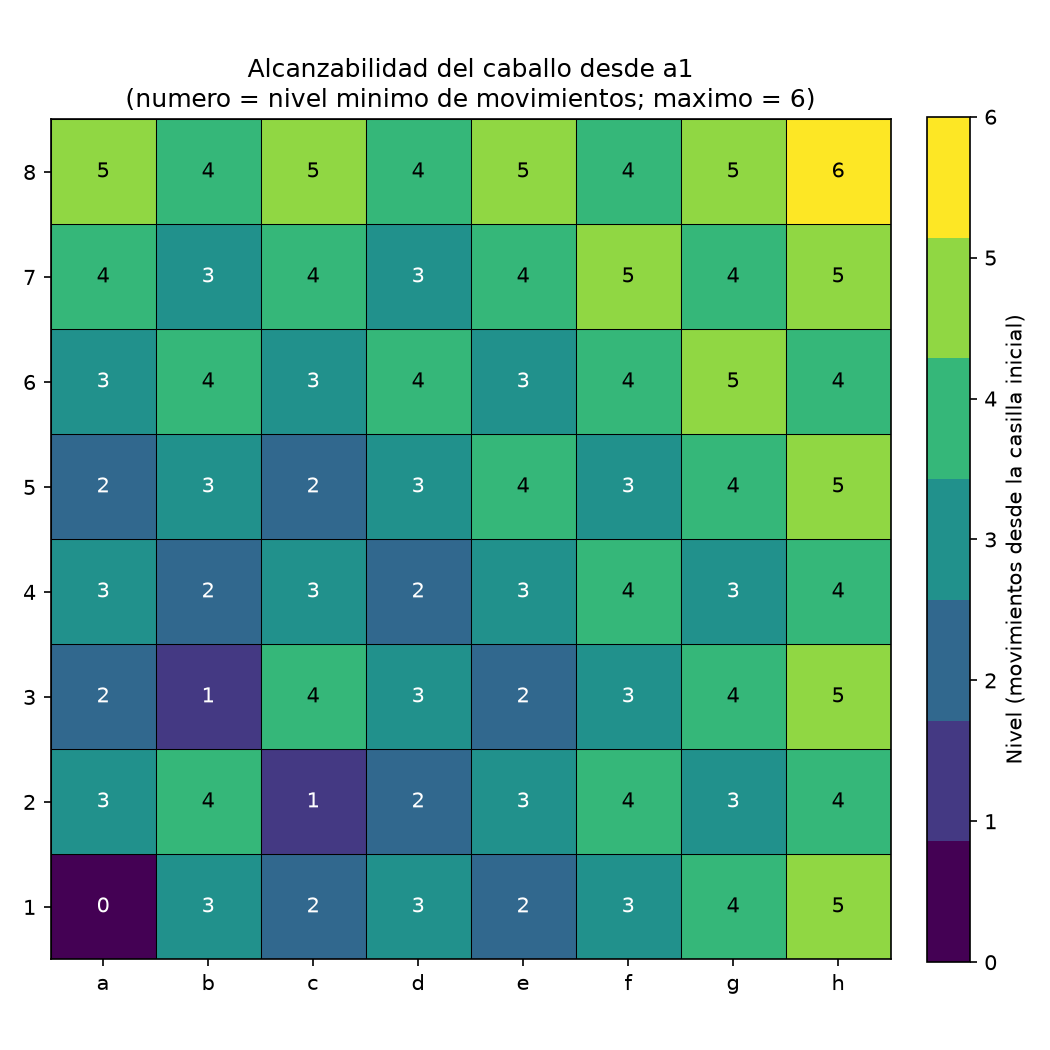
\includegraphics[width=0.7\textwidth]{../results/alcanzabilidad_a1.png}
\caption{Nivel de alcanzabilidad desde \(a1\).}
\label{fig:alcanzabilidad-a1}
\end{figure}

\subsection{Caso \texorpdfstring{\(d5\)}{d5}}

Partiendo de \(d5\), también se alcanzan las \textbf{64 casillas}, pero
en solo \textbf{4 niveles}: menos de la tercera parte de los niveles
requeridos desde \(a1\). La Figura~\ref{fig:alcanzabilidad-d5} muestra
el resultado.

\begin{figure}[H]
\centering
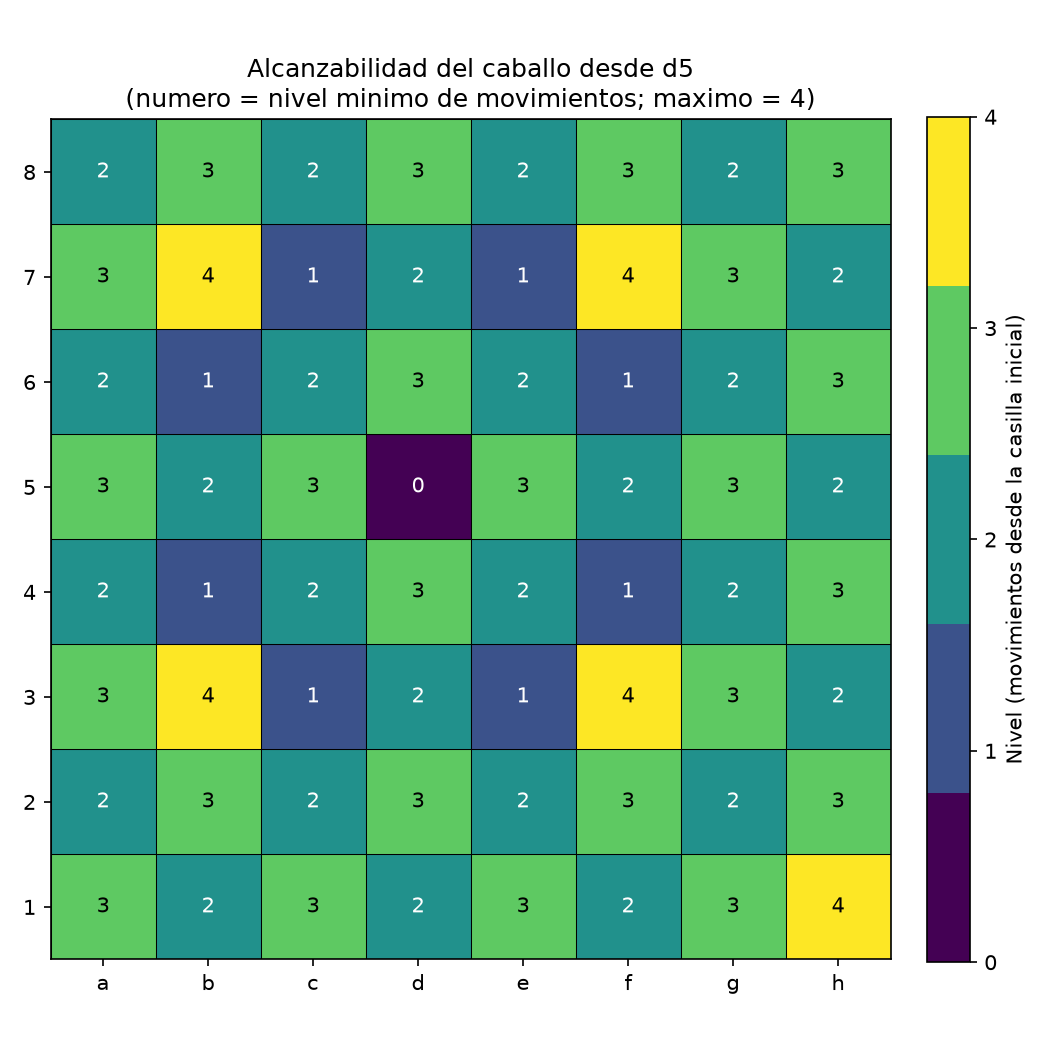
\includegraphics[width=0.7\textwidth]{../results/alcanzabilidad_d5.png}
\caption{Nivel de alcanzabilidad desde \(d5\).}
\label{fig:alcanzabilidad-d5}
\end{figure}

\subsection{Comparación}

La Tabla~\ref{tab:comparacion-bfs} resume ambos recorridos.

\begin{table}[H]
\centering
\caption{Comparación de la exploración por niveles desde \(a1\) y \(d5\).}
\label{tab:comparacion-bfs}

\begin{tabular}{lcc}
\toprule
 & Desde \(a1\) & Desde \(d5\) \\
\midrule
Casillas alcanzadas & 64 de 64 & 64 de 64 \\
Casillas no alcanzadas & 0 & 0 \\
Número de niveles & 6 & 4 \\
Casillas en el último nivel & 1 (\(h8\)) & 5 (\(b3,b7,f3,f7,h1\)) \\
\bottomrule
\end{tabular}

\end{table}

En ambos casos se alcanzan las 64 casillas, lo cual constituye la
verificación empírica, mediante dos puntos de partida distintos, de la
irreducibilidad discutida en la Sección~4.1: dado que el grafo de
movimientos es conexo, cualquier casilla inicial alcanza eventualmente
a todas las demás. La diferencia en el número de niveles requeridos
(6 frente a 4) se explica por la posición relativa de cada casilla:
\(a1\) es una esquina con solo \(|N(a1)|=2\), mientras que \(d5\) es
una casilla central con \(|N(d5)|=8\), lo que le permite ramificarse
mucho más rápidamente por el tablero. En términos de teoría de grafos,
\(d5\) tiene menor excentricidad que \(a1\) dentro del grafo de
movimientos del caballo.

% ------------------------------------------------
% 7. CONCLUSIONES
% ------------------------------------------------

\section{Conclusiones}

El movimiento aleatorio de un caballo sobre un tablero de ajedrez
\(8\times8\) define una cadena de Markov finita cuyas propiedades
pueden determinarse por completo mediante construcción y verificación
computacional. Se comprobó que la matriz de transición \(P\), aunque
construida a partir de una relación de movimientos simétrica, no es
en sí misma simétrica: la probabilidad de transición depende del grado
\(|N(x)|\) de la casilla de origen, no de la de destino.

El análisis de alcanzabilidad mostró que la cadena es irreducible:
cualquier casilla puede alcanzar a cualquier otra, aunque el número de
pasos necesarios varía considerablemente según la posición inicial
(6 niveles desde una esquina frente a 4 desde el centro). Un resultado
adicional, no exigido explícitamente por el enunciado pero relevante
para la caracterización completa de la cadena, es que esta resulta
\textbf{periódica con período 2}, consecuencia directa de que el grafo
de movimientos del caballo es bipartito respecto a la coloración
habitual del tablero de ajedrez. Esto implica que, a diferencia de una
cadena irreducible y aperiódica, \(P^n\) no converge puntualmente a una
matriz límite, aunque sí existe una única distribución estacionaria.

Finalmente, el cálculo de probabilidades sobre trayectorias específicas
ilustró de manera concreta la propiedad de Markov: tanto la
probabilidad de una trayectoria completa como la probabilidad
condicional a un estado intermedio se obtienen como productos simples
de entradas de \(P\), y la probabilidad de transición en dos pasos
calculada mediante \(P^2\) coincidió exactamente con la obtenida por
suma explícita sobre el estado intermedio, verificando computacionalmente
la identidad de Chapman--Kolmogorov.

% ------------------------------------------------
% 8. ANEXO
% ------------------------------------------------

\section{Anexo: código utilizado}

El código empleado para construir la cadena, calcular las
probabilidades y generar las figuras de este informe se encuentra
organizado en el directorio

\begin{center}
\texttt{tarea-02-caballo/src/}
\end{center}

dentro de la estructura del repositorio del curso, con módulos
independientes para la representación del tablero
(\texttt{tablero.py}), la construcción de la matriz de transición
(\texttt{matriz\_transicion.py}), el cálculo de probabilidades del
ejercicio 2 (\texttt{ejercicio2.py}), la exploración de alcanzabilidad
(\texttt{alcanzabilidad.py}) y la generación de figuras
(\texttt{visualizacion.py}). Cada módulo cuenta con pruebas
automatizadas correspondientes en \texttt{tarea-02-caballo/tests/}.

\url{https://github.com/Henry2899/cadenas-markov-aplicaciones}

\end{document}
